% !TeX program = xelatex
%%%%%%%%%%%%%%%%%%%%%%%%%%%%%%%%%%%%%%%%%%%%%%%%%%%%%%%%%%%%%%%%%%%%%%%%%%%%%%%%
%2345678901234567890123456789012345678901234567890123456789012345678901234567890
%        1         2         3         4         5         6         7         8

\documentclass[letterpaper, 10 pt, conference]{ieeeconf}  % Comment this line out if you need a4paper

%\documentclass[a4paper, 10pt, conference]{ieeeconf}      % Use this line for a4 paper

\IEEEoverridecommandlockouts                              % This command is only needed if 
                                                          % you want to use the \thanks command

\overrideIEEEmargins                                      % Needed to meet printer requirements.

%In case you encounter the following error:
%Error 1010 The PDF file may be corrupt (unable to open PDF file) OR
%Error 1000 An error occurred while parsing a contents stream. Unable to analyze the PDF file.
%This is a known problem with pdfLaTeX conversion filter. The file cannot be opened with acrobat reader
%Please use one of the alternatives below to circumvent this error by uncommenting one or the other
%\pdfobjcompresslevel=0
%\pdfminorversion=4

% See the \addtolength command later in the file to balance the column lengths
% on the last page of the document

% The following packages can be found on http:\\www.ctan.org
%\usepackage{graphics} % for pdf, bitmapped graphics files
%\usepackage{epsfig} % for postscript graphics files
%\usepackage{mathptmx} % assumes new font selection scheme installed
%\usepackage{times} % assumes new font selection scheme installed
%\usepackage{amsmath} % assumes amsmath package installed
%\usepackage{amssymb}  % assumes amsmath package installed

\usepackage{iftex}
\ifPDFTeX
  \usepackage[utf8]{inputenc}
  \usepackage[T1]{fontenc}
\else
  \usepackage{fontspec}
  \usepackage{xeCJK}
  \setCJKmainfont{Songti SC}
  \setCJKsansfont{Heiti SC}
  \setCJKmonofont{Songti SC}
  \XeTeXlinebreaklocale "zh"
  \XeTeXlinebreakskip=0pt plus 1pt
\fi
\usepackage{amsmath,amssymb}
\usepackage{graphicx}
\usepackage{booktabs}
\usepackage{xcolor}
\usepackage{cite}
\usepackage{hyperref}
\usepackage{url}
\usepackage{microtype}
\usepackage{algorithm}
\usepackage{algorithmic}
\usepackage{multirow}
\usepackage{balance}
\usepackage{tabularx}
\usepackage{array}


\title{\LARGE \bf
Preparation of Papers for IEEE Sponsored Conferences \& Symposia*
}


\author{Albert Author$^{1}$ and Bernard D. Researcher$^{2}$% <-this % stops a space
\thanks{*This work was not supported by any organization}% <-this % stops a space
\thanks{$^{1}$Albert Author is with Faculty of Electrical Engineering, Mathematics and Computer Science,
        University of Twente, 7500 AE Enschede, The Netherlands
        {\tt\small albert.author@papercept.net}}%
\thanks{$^{2}$Bernard D. Researcheris with the Department of Electrical Engineering, Wright State University,
        Dayton, OH 45435, USA
        {\tt\small b.d.researcher@ieee.org}}%
}


\begin{document}



\maketitle
\thispagestyle{empty}
\pagestyle{empty}


%%%%%%%%%%%%%%%%%%%%%%%%%%%%%%%%%%%%%%%%%%%%%%%%%%%%%%%%%%%%%%%%%%%%%%%%%%%%%%%%
\begin{abstract}

This electronic document is a ÒliveÓ template. The various components of your paper [title, text, heads, etc.] are already defined on the style sheet, as illustrated by the portions given in this document.

\end{abstract}


%%%%%%%%%%%%%%%%%%%%%%%%%%%%%%%%%%%%%%%%%%%%%%%%%%%%%%%%%%%%%%%%%%%%%%%%%%%%%%%%
\section{INTRODUCTION}

Wide-angle central cameras, such as fisheye cameras, capture a
larger angular extent of the scene within a single image, providing
broader visual coverage for geometric vision tasks such as visual
odometry and 3D reconstruction. However, fully exploiting these
additional observations requires an accurate geometric calibration
over the entire image domain, especially in peripheral regions where
the projection behavior changes significantly. Compared with
conventional cameras, wide-angle cameras introduce two major
challenges in calibration: First, the strong nonlinearity of the projection model makes model
selection, parameter initialization, and nonlinear optimization more
difficult~\cite{polic2020uncertainty,lochman2021babelcalib}. Second, severe projection
variation and image deformation near the image boundary reduce the
reliability of target detection and feature localization~\cite{duisterhof2022tartancalib}. Accordingly, existing work has
largely proceeded along two complementary directions: designing more suitable wide-angle camera models
~\cite{kannala2006generic,usenko2018double}, and improving the quality of calibration
observations through target design, feature refinement, and
view or observation selection
~\cite{ha2017deltille,peng2019calibration,
duisterhof2022tartancalib,liu2026observation}.

This work focuses on the latter direction and investigates how
planar calibration targets can provide more effective geometric
constraints. Camera calibration typically estimates camera intrinsics
and target poses from image observations of a target with known
geometry. Planar targets such as checkerboards and AprilGrids are
widely used due to their simple structures and convenient feature
detection~\cite{zhang2000flexible,olson2011apriltag}. For conventional lenses, translating and rotating a single
planar target can provide sufficient observations to constrain
the camera model. However, wide-angle cameras are more sensitive to
the distribution of calibration observations. When observations are
limited to a narrow radial range, the focal scale and projection-shape parameters can induce
similar residual variations, leading to poorly separated parameter
directions and ill-conditioned linearized updates
~\cite{liu2026observation}.
Therefore, wide-angle calibration requires not only a sufficient
number of features, but also observations spanning different radial
regions to provide more discriminative geometric constraints for
camera model estimation.

However, realizing broad radial coverage with a single planar target is
difficult in practice. In each view, a single target occupies only a
limited and continuous image region, and its radial coverage is bounded
by its projected extent. Enlarging the target projection increases the
radial span, but also forces the same pattern to cross image regions
with substantially different projection scales and distortion levels,
placing greater demands on feature detection and subpixel localization.
Existing wide-angle calibration methods mitigate this problem by using
an intermediate camera model to reproject the target and adaptively
refine missing or distorted features. Nevertheless, a practical trade-off
remains between radial coverage and local observation reliability. This
motivates a calibration framework that distributes reliable observations
across different field-of-view regions while preserving stable local
feature detection.

Motivated by these findings, we construct a distributed multi-board
target using multiple boards, each carrying a uniquely coded AprilTag.
The boards can be independently detected and associated within the same
image, allowing observations to be distributed across different spatial
and radial regions without requiring a single large continuous target to
span the strongly distorted image domain. Each tag directly provides
four sparse observations, referred to as outer corners. Although
these distributed outer corners are sufficient to bootstrap an
intermediate camera model, they remain locally sparse for final
calibration. We therefore use the intermediate model to predict the
image locations of predefined internal lattice points and refine them
using local image evidence. In this way, spatially distributed but
locally sparse outer-corner observations are extended into dense and
geometrically consistent observations across different field-of-view
regions. Based on this design, we develop a multi-board calibration
system for wide-angle central cameras that integrates distributed target
detection, dense observation recovery, and camera calibration into a
unified pipeline.

Our main contributions are summarized as follows:

\begin{itemize}
\setlength{\itemsep}{1pt}
\setlength{\parskip}{0pt}
\setlength{\parsep}{0pt}
\item We present an open-source, easy-to-deploy, and flexible multi-board
calibration system for wide-angle central cameras.
\item To address insufficient spatial coverage of calibration observations
 and unreliable feature refinement, we propose a distributed multi-board 
 design based on single AprilTags, together with an intermediate-model-ass
 isted internal lattice-point refinement method. On the evaluated sequence,
  the distributed design improves occupied-grid coverage by $14.6$ percentage points under the same frame--board budget.
\item We conduct a controlled analysis that isolates the contribution
of recovered internal lattice observations under an identical Outer4
initialization. The results show that local observation densification
provides complementary constraints for more faithful estimation of the
wide-angle projection model.
\end{itemize}

Tests on several datasets and camera models cover reprojection error, ablations,
cross-backend calibration, and held-out pose estimation. The results show
reliable calibration and competitive accuracy.

\section{}

\subsection{Selecting a Template (Heading 2)}

First, confirm that you have the correct template for your paper size. This template has been tailored for output on the US-letter paper size. 
It may be used for A4 paper size if the paper size setting is suitably modified.

\subsection{Maintaining the Integrity of the Specifications}

The template is used to format your paper and style the text. All margins, column widths, line spaces, and text fonts are prescribed; please do not alter them. You may note peculiarities. For example, the head margin in this template measures proportionately more than is customary. This measurement and others are deliberate, using specifications that anticipate your paper as one part of the entire proceedings, and not as an independent document. Please do not revise any of the current designations

\section{Method}

\subsection{Multi-Board Target Formulation}

Our calibration target consists of $N$ rigid boards, each carrying a
uniquely coded AprilTag:
\begin{equation}
\mathcal{B}=\{B_0,B_1,\ldots,B_{N-1}\},
\end{equation}
where $B_0$ is selected as the reference board. Let
$\mathcal{F}_{B_b}$ denote the local coordinate frame of board $B_b$,
and let $\mathbf{p}_{b,j}\in\mathbb{R}^3$ denote the $j$-th target point
expressed in $\mathcal{F}_{B_b}$. The target points include the directly
detected outer corners and the internal lattice points recovered in
Sec.~\ref{sec:internal_point_recovery}.

We use $\mathcal{F}_{B_0}$ as the common coordinate frame of the
multi-board target and fix
$\mathbf{T}_{B_0B_0}=\mathbf{I}$.
Let $\mathbf{T}_{B_0B_b}\in SE(3)$ denote the static rigid transform
from $\mathcal{F}_{B_b}$ to $\mathcal{F}_{B_0}$. For frame $t$, let
$\mathcal{F}_{C_t}$ be the camera coordinate frame and let
$\mathbf{T}_{C_tB_0}\in SE(3)$ denote the pose of the reference board
in $\mathcal{F}_{C_t}$. A point on board $B_b$ is therefore
expressed in the camera frame as
\begin{equation}
\mathbf{x}_{t,b,j}
=
\mathbf{T}_{C_tB_0}
\mathbf{T}_{B_0B_b}
\mathbf{p}_{b,j}.
\end{equation}

Given the camera parameters $\boldsymbol{\theta}$ and the projection
function $\pi(\cdot;\boldsymbol{\theta})$, the predicted image
location is
\begin{equation}
\hat{\mathbf{u}}_{t,b,j}
=
\pi\!\left(
\mathbf{x}_{t,b,j};
\boldsymbol{\theta}
\right)
=
\pi\!\left(
\mathbf{T}_{C_tB_0}
\mathbf{T}_{B_0B_b}
\mathbf{p}_{b,j};
\boldsymbol{\theta}
\right).
\end{equation}
The corresponding image observation is denoted by
$\mathbf{u}_{t,b,j}\in\mathbb{R}^2$. We collect all valid
observations in
\begin{equation}
\mathcal{O}
=
\left\{
(t,b,j,\mathbf{u}_{t,b,j})
\right\}.
\end{equation}
The unknown variables comprise the camera parameters
$\boldsymbol{\theta}$, the per-frame reference-board poses
$\{\mathbf{T}_{C_tB_0}\}$, and the static inter-board transforms
$\{\mathbf{T}_{B_0B_b}\}_{b=1}^{N-1}$.

\subsection{Camera Model Initialization}

At the beginning of calibration, no reliable camera model is available,
while a usable initialization is important for nonlinear wide-angle
calibration. The distributed AprilTag boards provide robust outer-corner
observations across different image and radial regions. We use these
observations to initialize the camera model. For a given camera-model
family, we construct an initial parameter vector
$\boldsymbol{\theta}^{0}$ using the image resolution and model-specific
default values.

For board $B_b$ observed in frame $t$, let
$\mathcal{C}^{\mathrm{out}}_{t,b}$ denote its valid outer-corner
observations. We define the reprojection residual as
\begin{equation}
\mathbf{r}^{\mathrm{out}}_{t,b,j}
(\boldsymbol{\theta},\mathbf{T})
=
\mathbf{u}_{t,b,j}
-
\pi\!\left(
\mathbf{T}\mathbf{p}_{b,j};
\boldsymbol{\theta}
\right).
\end{equation}
Given $\boldsymbol{\theta}^{0}$, a temporary frame--board pose is
initialized by
\begin{equation}
\widetilde{\mathbf{T}}^{0}_{C_tB_b}
=
\operatorname*{arg\,min}_{\mathbf{T}\in SE(3)}
\sum_{j\in\mathcal{C}^{\mathrm{out}}_{t,b}}
\left\|
\mathbf{r}^{\mathrm{out}}_{t,b,j}
(\boldsymbol{\theta}^{0},\mathbf{T})
\right\|_2^2 .
\end{equation}

We perform this initialization independently for all valid frame--board
observations and reject estimates with invalid poses or excessive
reprojection errors. Let $\mathcal{S}$ denote the retained frame--board
pairs. We then jointly refine the camera parameters and temporary poses:
\begin{equation}
\begin{aligned}
&\boldsymbol{\theta}^{*},
\left\{
\widetilde{\mathbf{T}}^{*}_{C_tB_b}
\right\}
\\
&\quad =
\operatorname*{arg\,min}_{
\boldsymbol{\theta},
\{\widetilde{\mathbf{T}}_{C_tB_b}\}}
\sum_{(t,b)\in\mathcal{S}}
\sum_{j\in\mathcal{C}^{\mathrm{out}}_{t,b}}
\rho\!\left(
\left\|
\mathbf{r}^{\mathrm{out}}_{t,b,j}
\left(
\boldsymbol{\theta},
\widetilde{\mathbf{T}}_{C_tB_b}
\right)
\right\|_2^2
\right).
\end{aligned}
\end{equation}
where $\rho(\cdot)$ is a robust loss function. At this stage, the boards
are not coupled through the unknown inter-board geometry; each valid
frame--board observation is assigned an independent pose. The optimized
parameters $\boldsymbol{\theta}^{*}$ initialize the subsequent complete
multi-board calibration and serve as the intermediate camera model for
internal-point recovery.

\subsection{Internal Lattice Point Recovery}
\label{sec:internal_point_recovery}

The outer corners provide stable board localization and are sufficient
to bootstrap an intermediate camera model. However, the four
observations from each tag remain locally sparse for final calibration.
We therefore use the intermediate model to recover image observations
for predefined internal lattice points, combining model-guided
prediction with local image evidence.

Given the intermediate camera parameters $\boldsymbol{\theta}^{*}$,
we reuse the temporary frame--board pose
$\widetilde{\mathbf{T}}^{*}_{C_tB_b}$ obtained in Sec.~\ref{sec:camera_init}.
For an internal lattice point
$\mathbf{p}_{b,j}$, $j\in\mathcal{C}^{\mathrm{int}}_b$, its direct
geometric projection
\begin{equation}
\widehat{\mathbf{u}}^{\mathrm{nom}}_{t,b,j}
=
\pi\!\left(
\widetilde{\mathbf{T}}^{*}_{C_tB_b}
\mathbf{p}_{b,j};
\boldsymbol{\theta}^{*}
\right)
\label{eq:nominal_internal_prediction}
\end{equation}
provides a nominal prediction and is used as a fallback when the
boundary-based seed described below is unavailable.

To construct the primary seed, we sample support points along the four
observed tag boundaries and back-project them onto the unit sphere using
the intermediate camera model. The resulting top, bottom, left, and
right boundary-ray curves are denoted by
$\mathbf{r}_{T}(s)$, $\mathbf{r}_{B}(s)$,
$\mathbf{r}_{L}(t)$, and $\mathbf{r}_{R}(t)$, respectively.
Let $(s_j,t_j)\in[0,1]^2$ be the normalized horizontal and vertical
coordinates of $\mathbf{p}_{b,j}$ on the board lattice. We interpolate
the opposite boundary curves as
\begin{equation}
\begin{aligned}
\mathbf{r}_{v}
&=
\operatorname{slerp}\!\left(
\mathbf{r}_{T}(s_j),
\mathbf{r}_{B}(s_j),
t_j
\right),\\
\mathbf{r}_{h}
&=
\operatorname{slerp}\!\left(
\mathbf{r}_{L}(t_j),
\mathbf{r}_{R}(t_j),
s_j
\right).
\end{aligned}
\label{eq:spherical_boundary_interpolation}
\end{equation}
The two interpolated rays are blended and projected back to the image:
\begin{equation}
\widetilde{\mathbf{d}}^{\mathrm{int}}_{t,b,j}
=
\frac{\mathbf{r}_{v}+\mathbf{r}_{h}}
{\left\|\mathbf{r}_{v}+\mathbf{r}_{h}\right\|_2},
\qquad
\widetilde{\mathbf{u}}^{\mathrm{int}}_{t,b,j}
=
\pi\!\left(
\widetilde{\mathbf{d}}^{\mathrm{int}}_{t,b,j};
\boldsymbol{\theta}^{*}
\right).
\label{eq:internal_point_seed}
\end{equation}

Starting from $\widetilde{\mathbf{u}}^{\mathrm{int}}_{t,b,j}$, we
perform a local search in the viewing-ray domain and then refine the
candidate to subpixel accuracy in the original image. A recovered
observation is rejected if it falls outside the image, lacks sufficient
local image evidence, or deviates from its seed by more than a predefined
threshold. Each accepted observation retains its board and lattice-point
indices and is added to $\mathcal{O}$ for joint optimization together
with the outer corners.

\subsection{Spherical Bundle Adjustment}

Standard bundle adjustment minimizes reprojection errors in the image
plane. For wide-angle cameras, however, the ray deviation corresponding
to a pixel residual depends on the image location and the local Jacobian
of the projection model. We therefore provide optional ray-domain and
hybrid objectives for final refinement.

Given an image observation $\mathbf{u}_{t,b,j}$, we back-project it
using the current camera parameters and normalize it to obtain the
observed ray:
\begin{equation}
\mathbf{d}^{\mathrm{obs}}_{t,b,j}
=
\frac{
\pi^{-1}(\mathbf{u}_{t,b,j};
\boldsymbol{\theta})
}{
\left\|
\pi^{-1}(\mathbf{u}_{t,b,j};
\boldsymbol{\theta})
\right\|_2
}.
\end{equation}
The corresponding predicted ray is obtained from the transformed target
point defined in Sec.~IV-A:
\begin{equation}
\mathbf{d}^{\mathrm{pred}}_{t,b,j}
=
\frac{\mathbf{x}_{t,b,j}}
{\|\mathbf{x}_{t,b,j}\|_2}.
\end{equation}
Let $\mathbf{B}_{t,b,j}\in\mathbb{R}^{3\times2}$ be an orthonormal
tangent basis at $\mathbf{d}^{\mathrm{obs}}_{t,b,j}$. The local ray
residual is defined as
\begin{equation}
\mathbf{r}^{\mathrm{ray}}_{t,b,j}
=
\mathbf{B}_{t,b,j}^{\top}
\left(
\mathbf{d}^{\mathrm{pred}}_{t,b,j}
-
\mathbf{d}^{\mathrm{obs}}_{t,b,j}
\right).
\end{equation}
This two-dimensional residual preserves the tangential degrees of
freedom of the ray discrepancy and provides a first-order approximation
of angular error in the small-residual regime. The observed ray and its
tangent basis are updated together with the camera parameters during
optimization.

We additionally define a normalized hybrid residual that balances the
pixel reprojection residual $\mathbf{r}^{\mathrm{px}}_{t,b,j}$ and the
ray residual:
\begin{equation}
\mathbf{r}^{\mathrm{hyb}}_{t,b,j}
=
\begin{bmatrix}
\sqrt{1-\lambda}\,
\mathbf{r}^{\mathrm{px}}_{t,b,j}/s_{\mathrm{px}}
\\
\sqrt{\lambda}\,
\mathbf{r}^{\mathrm{ray}}_{t,b,j}/s_{\mathrm{ray}}
\end{bmatrix},
\qquad
\lambda\in[0,1],
\end{equation}
where $s_{\mathrm{px}}$ and $s_{\mathrm{ray}}$ are fixed normalization
scales computed from the median residual magnitudes before final
refinement. The standard pixel objective is used by default, while the
ray-domain and hybrid objectives are provided as optional final
refinement alternatives.

\section{EXPERIMENT}

\begin{figure}[t]
  \centering
  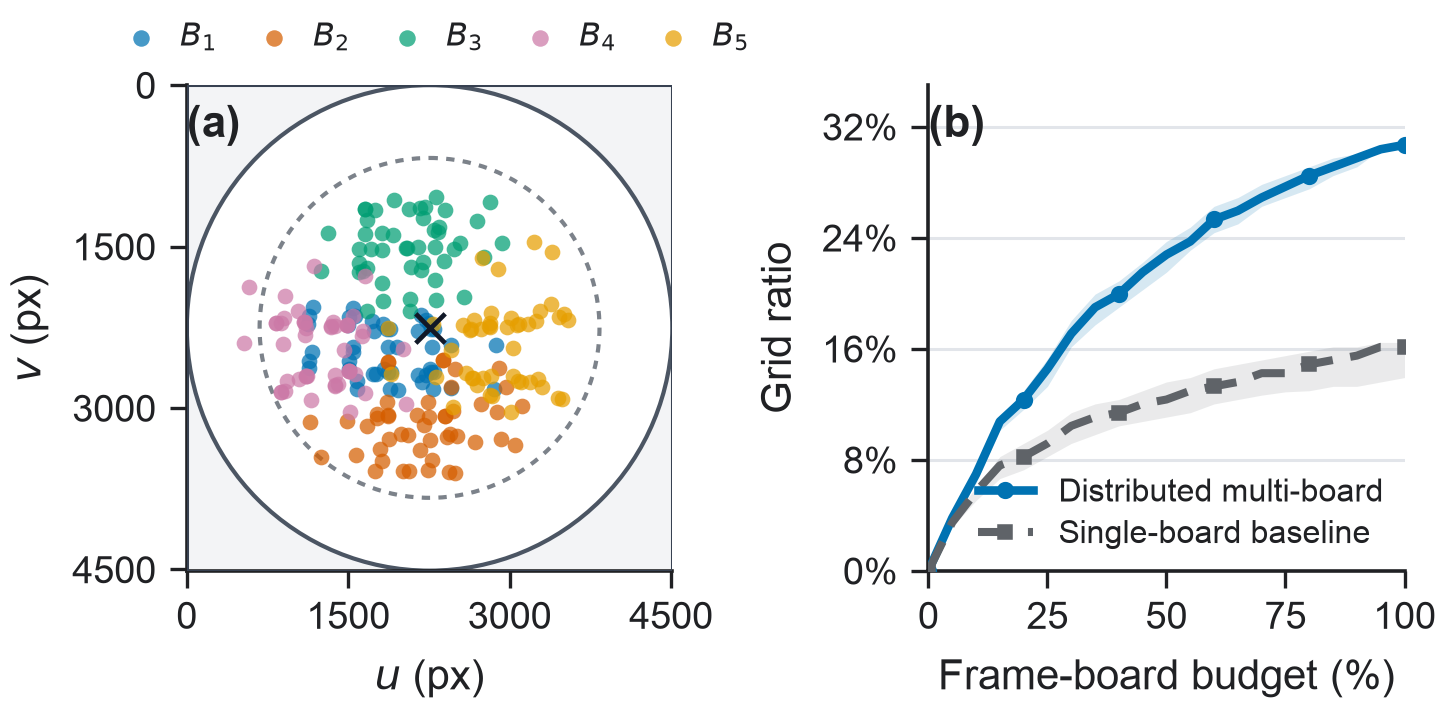
\includegraphics[width=\linewidth]{pic/corner_distribution_and_coverage_efficiency.png}
  \caption{xxxxxx}
  \label{fig:corner_distribution}
\end{figure}

\begin{table*}[t]
\centering
\caption{
Cross-backend verification on the held-out multi-board and independent
checkerboard test sets. BabelCalib uses the same detected observations
and target geometry as ours.
}
\label{tab:cross_backend_verification}

\footnotesize
\setlength{\tabcolsep}{3.2pt}
\renewcommand{\arraystretch}{1.08}

\begin{tabularx}{\textwidth}{
@{}
l
>{\raggedright\arraybackslash}p{3.75cm}
@{\hspace{1pt}}
c
c
>{\centering\arraybackslash}X
c
c
@{}
}
\toprule
\multirow{2}{*}{Model}
& \multirow{2}{*}{Method / Observations}
& \multirow{2}{*}{$f_u / f_v$}
& \multirow{2}{*}{$c_u / c_v$}
& \multirow{2}{*}{Model Params.}
& \multicolumn{2}{c}{Test RMSE [px] $\downarrow$} \\
\cmidrule(lr){6-7}
&
&
&
&
& Multi-board
& Checkerboard \\
\midrule

\multirow{3}{*}{DS}
& Ours
& 1175.65 / 1175.29
& 2242.88 / 2275.61
& $[-0.1905,\ 0.6171]$
& \textbf{0.5228}
& \textbf{0.5918} \\

& BabelCalib w/ Outer+Internal
& 1176.56 / 1175.92
& 2242.90 / 2275.63
& $[-0.1914,\ 0.6175]$
& 0.5293
& 0.6020 \\

& BabelCalib w/ Outer4 only
& 1943.49 / 1943.08
& 2242.91 / 2275.67
& $[0.3401,\ 0.8048]$
& $0.5256^{\dagger}$
& -- \\

\midrule

\multirow{3}{*}{KB}
& Ours
& 1451.58 / 1451.10
& 2242.37 / 2275.38
& $[-0.0197,\ 0.0010,\ -0.0032,\ 0.0006]$
& \textbf{0.5216}
& \textbf{0.5960} \\

& BabelCalib w/ Outer+Internal
& 1454.52 / 1453.74
& 2242.91 / 2275.65
& $[-0.0196,\ -0.0018,\ -0.0007,\ -0.0001]$
& 0.5286
& 0.6052 \\

& BabelCalib w/ Outer4 only
& --
& --
& --
& --
& -- \\

\bottomrule
\end{tabularx}

\vspace{2pt}
\parbox{\textwidth}{
\scriptsize
$^\dagger$ The Outer4-only setting achieves a comparable multi-board
test RMSE but converges to a substantially shifted intrinsic parameterization.
}
\end{table*}

\begin{table}[t]
\centering
\caption{Internal-seed ablation with a shared Outer4 initialization.}
\label{tab:internal_seed_ablation}
\footnotesize
\setlength{\tabcolsep}{1.5pt}
\renewcommand{\arraystretch}{1.05}
\begin{tabular}{@{}lcccc@{}}
\toprule
Method
& \shortstack{Reproj.\\[-1pt]Err. [px] $\downarrow$}
& \shortstack{Outer\\[-1pt]Err. [px] $\downarrow$}
& \shortstack{Internal\\[-1pt]Err. [px] $\downarrow$}
& \shortstack{Max.\\[-1pt]Err. [px] $\downarrow$} \\
\midrule
Outer-only & 0.5251 & \textbf{0.1002} & 0.5582 & 1.679 \\
Virtual Pinhole Patch & 4.3647 & 0.1089 & 4.6499 & 50.353 \\
\textbf{Spherical Seed} & \textbf{0.5243} & 0.1030 & \textbf{0.5572} & \textbf{1.678} \\
\bottomrule
\end{tabular}
\vspace{2pt}
\parbox{\columnwidth}{\scriptsize \textit{Note.} Spherical Seed is our method. Internal error uses frozen validation points excluded from Outer-only optimization; max. error is the maximum frame--board RMSE.}
\end{table}

\subsection{Experimental Setup}


\subsection{Ablation}
This section evaluates two aspects of the recovered internal lattice
observations: their generation reliability and their constraining effect
on camera calibration. We first compare internal-seed constructions in
different geometric domains, and then examine whether the recovered
internal observations improve intrinsic recovery.

\subsubsection{Internal Seed Generation}

Given accurate outer-corner detections, internal-point refinement
depends on the geometric quality of the initial seeds. We compare two
strategies: Virtual Pinhole Patch and Spherical Seed. Following
TartanCalib, Virtual Pinhole Patch uses an intermediate camera model to
remap the wide-FoV image into virtual pinhole views. In contrast,
Spherical Seed constructs the seeds directly in the viewing-ray domain
via spherical interpolation. Both variants use the same Outer4
initialization, local refinement, and optimization backend. We also
include Outer-only as a baseline without internal-point recovery.

Table~\ref{tab:internal_seed_ablation} summarizes the results. Virtual
Pinhole Patch achieves an outer error comparable to Spherical Seed, but
produces substantially larger internal and maximum errors, increasing
the overall reprojection error. Since the two variants share the same
Outer4 initialization, the degradation mainly arises from unreliable
internal seeds. In contrast, Spherical Seed maintains an overall error
comparable to Outer-only while incorporating additional internal
observations, indicating that viewing-ray-domain seed construction is
more consistent with wide-FoV projection geometry.

\subsubsection{Internal Observation Evaluation}

The preceding experiment shows that Spherical Seed can reliably recover
internal observations. However, because it shares the same Outer4
initialization with Outer-only, both settings start from a nearly
converged model. Their final reprojection errors therefore cannot isolate
the contribution of internal lattice points to intrinsic recovery. To
directly evaluate this contribution, we construct a controlled
intrinsic-recovery experiment using the Double Sphere (DS) model. Both
settings share the same reference scene, perturbed initialization,
Outer4 frame--board observations, and paired noise realizations;
Outer+Internal additionally incorporates only the internal lattice
points recovered by Spherical Seed.

In wide-FoV calibration, limited radial coverage may cause focal scale
and projection-shape parameters to induce similar residual changes.
Rather than arbitrarily perturbing an individual intrinsic parameter,
we extract the least-constrained intrinsic direction
$\mathbf{d}_{W_1}$ from the pose-eliminated Schur information matrix
computed using the full-budget Outer-only observations. This direction
is fixed for both settings and across all observation budgets. For
method $m$ and budget $b$, the information along this direction is
defined as
\begin{equation}
I_{W_1}^{m,b}
=
\mathbf{d}_{W_1}^{\top}
\mathbf{S}_c^{m,b}
\mathbf{d}_{W_1}.
\end{equation}

We then perturb the reference DS intrinsics along this direction such
that the initial model has a P95 ray error of $2^\circ$ in the
peripheral region $\rho \geq 0.7$. Fig.~\ref{fig:internal-point-ablation}
evaluates the information along the weakest intrinsic direction, the
model-recovery error over the full FoV, and the observation budget
required to reach the prescribed peripheral-accuracy target.

We then perturb the reference DS intrinsics along
$\mathbf{d}_{W_1}$ such that the initial model reaches a P95 ray error
of $2^\circ$ in the peripheral region $\rho \geq 0.7$.
Fig.~\ref{fig:internal-point-ablation} compares the information along
the weakest intrinsic direction, the model-recovery error over the full
FoV, and the observation budget required to reach the prescribed
peripheral-accuracy target.

As shown in Fig.~\ref{fig:internal-point-ablation}(a), incorporating
internal lattice points consistently strengthens the constraint along
the weakest intrinsic direction across all frame--board budgets.
Fig.~\ref{fig:internal-point-ablation}(b) shows that the recovered model
more closely matches the reference model over the full FoV, with larger
improvements near the image periphery.
Fig.~\ref{fig:internal-point-ablation}(c) further shows that
Outer+Internal reaches the prescribed peripheral-accuracy target with
fewer observations. These results indicate that internal lattice points
do not replace the initialization provided by spatially distributed
Outer4 observations. Instead, they provide complementary local
constraints that improve DS model recovery in highly distorted
peripheral regions.

\begin{figure*}[t]
  \centering
  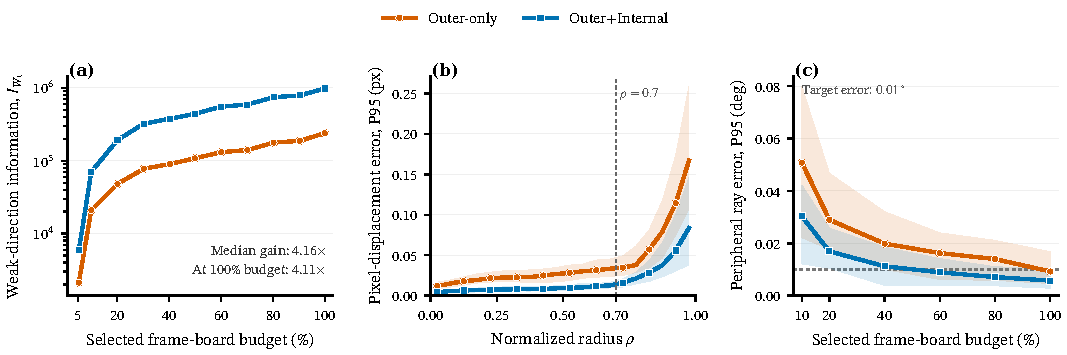
\includegraphics[width=0.98\textwidth]{pic/internal_point_ablation.pdf}
  \caption{Effect of internal observations on the recovery of perturbed
  DS intrinsics. Outer-only and Outer+Internal share the same Outer4
  frame--board observations, perturbed initialization, and paired noise
  realizations; Outer+Internal additionally incorporates the recovered
  internal lattice points.
  (a) Schur information along the least-constrained intrinsic direction
  $W_1$ after pose elimination.
  (b) P95 radial pixel displacement between the recovered and reference
  models, evaluated on a fixed grid of reference rays.
  (c) Peripheral P95 ray error under different frame--board budgets.
  Both settings start from the same $2^\circ$ peripheral perturbation
  and optimize only the DS intrinsics. Panels (b) and (c) summarize
  100 paired trials; the curves and shaded regions denote the median
  and interquartile range (IQR), respectively. The peripheral region is
  defined as $\rho \geq 0.7$.}
  \label{fig:internal-point-ablation}
\end{figure*}

\subsection{Camera Pose Estimation}

To evaluate the calibration results, we perform camera pose estimation
on held-out test images. The images are randomly split into training
and test sets at a ratio of $7{:}3$.For each method, we fix the evaluated camera intrinsics
and the shared multi-board geometry during testing, and optimize only
the pose of the reference board with respect to the camera by minimizing
a robust reprojection objective. Reprojection errors are then evaluated
over all visible board observations in each image using RMSE, P95, and
Inlier@1px.

Since the compared calibration pipelines are not directly applicable
to our multi-board calibration setup, we estimate their camera
intrinsics using standard checkerboard-based calibration procedures.
The resulting intrinsics are then evaluated alongside ours on the same
held-out multi-board pose-estimation task and are reported as reference
baselines 

\section{CONCLUSIONS}

A conclusion section is not required. Although a conclusion may review the main points of the paper, do not replicate the abstract as the conclusion. A conclusion might elaborate on the importance of the work or suggest applications and extensions. 

\addtolength{\textheight}{-12cm}   % This command serves to balance the column lengths
                                  % on the last page of the document manually. It shortens
                                  % the textheight of the last page by a suitable amount.
                                  % This command does not take effect until the next page
                                  % so it should come on the page before the last. Make
                                  % sure that you do not shorten the textheight too much.

%%%%%%%%%%%%%%%%%%%%%%%%%%%%%%%%%%%%%%%%%%%%%%%%%%%%%%%%%%%%%%%%%%%%%%%%%%%%%%%%



%%%%%%%%%%%%%%%%%%%%%%%%%%%%%%%%%%%%%%%%%%%%%%%%%%%%%%%%%%%%%%%%%%%%%%%%%%%%%%%%



%%%%%%%%%%%%%%%%%%%%%%%%%%%%%%%%%%%%%%%%%%%%%%%%%%%%%%%%%%%%%%%%%%%%%%%%%%%%%%%%
\section*{APPENDIX}

Appendixes should appear before the acknowledgment.

\section*{ACKNOWLEDGMENT}

The preferred spelling of the word ÒacknowledgmentÓ in America is without an ÒeÓ after the ÒgÓ. Avoid the stilted expression, ÒOne of us (R. B. G.) thanks . . .Ó  Instead, try ÒR. B. G. thanksÓ. Put sponsor acknowledgments in the unnumbered footnote on the first page.



%%%%%%%%%%%%%%%%%%%%%%%%%%%%%%%%%%%%%%%%%%%%%%%%%%%%%%%%%%%%%%%%%%%%%%%%%%%%%%%%

References are important to the reader; therefore, each citation must be complete and correct. If at all possible, references should be commonly available publications.



\bibliographystyle{IEEEtran}
\bibliography{references}



\end{document}
